% !TEX root = ../../presentation.tex
% Architektur: Implementierung

\begin{frame}[fragile]{Implementierung einer Instruktion}
  \pause
  \begin{lstlisting}[style=C++,emph={getValue, validate, assemble},emphstyle=\underline]
    class AbstractSyntaxTreeNode {
     public:
      using Node = std::shared_ptr<AbstractSyntaxTreeNode>;

      virtual MemoryValue
      getValue(MemoryAccess& memoryAccess) const = 0;

      virtual ValidationResult
      validate(MemoryAccess& memoryAccess) const = 0;

      virtual MemoryValue assemble() const = 0;
      
     protected:
      std::vector<Node> _children;
    };
  \end{lstlisting}
\end{frame}

% Anmerkung: in RISC-V ist der AST nie tiefer als 2 Knoten

\begin{slide}{\texttt{getValue()}}
  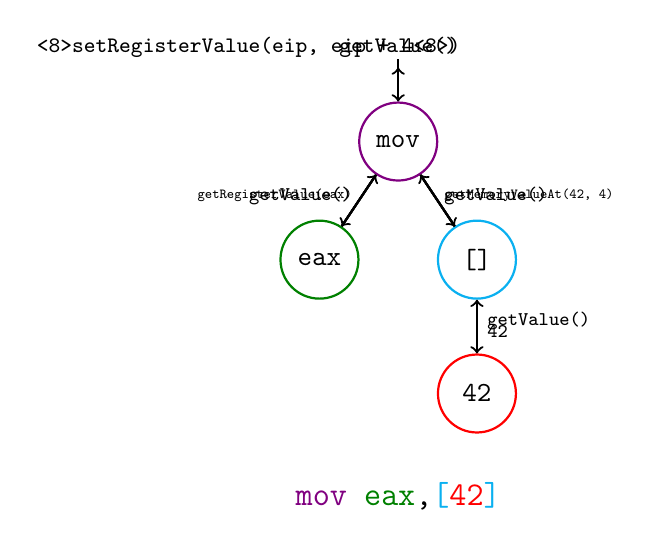
\begin{tikzpicture}[thick]
    \tikzset{node/.style={draw, circle, inner sep=0.35cm}};

    % Nodes
    \path (0, 0) coordinate [Purple, node] (mov) node {\texttt{mov}};
    \path (-1, -1.5) coordinate [Green, node] (eax) node {\texttt{eax}};
    \path (+1, -1.5) coordinate [ProcessBlue, node] (mem) node {\texttt{[]}};
    \path (+1, -3.2) coordinate [Red, node] (42) node {\texttt{42}};

    % Edges
    \draw (mov) -- (eax);
    \draw (mov) -- (mem);
    \draw (mem) -- (42);

    % Code
    \draw (0, -4.5) node {\large\texttt{%
      \textcolor{Purple}{mov} \textcolor{Green}{eax},%
      \textcolor{ProcessBlue}{[}\textcolor{Red}{42}\textcolor{ProcessBlue}{]}}%
    };

    % getValue() calls
    \onslide<2-6>{
      \node (getValue) at (0, 1.2) {\footnotesize\texttt{getValue()}};
      \draw [->, shorten <= -3pt] (getValue) -- (mov);
    }

    \onslide<3-5>{
      \draw [->] (mov) -- (eax)
            node [pos=0.4, left] {\scriptsize\texttt{getValue()}};
      \draw [->] (mov) -- (mem)
            node [pos=0.4, right] {\scriptsize\texttt{getValue()}};
    }

    \onslide<4>{
      \draw [->] (mem) -- (42)
            node [pos=0.4, right] {\scriptsize\texttt{getValue()}};
    }

    % getValue() results
    \onslide<5->{
    \draw [->] (42) -- (mem)
          node [pos=0.4, right] {\scriptsize\texttt{42}};
    }

    \onslide<6->{
      \draw [->] (eax) -- (mov)
            node [pos=0.6, left]
            {\tiny\texttt{getRegisterValue(eax)}};
      \draw [->] (mem) -- (mov)
            node [pos=0.6, right]
            {\tiny\texttt{getMemoryValueAt(42, 4)}};
    }

    \onslide<7->{
      \draw [->] (mov) -- (getValue);
      \node (getValue) at (-1.9, 1.2) {%
        \footnotesize\texttt{%
        \onslide<8>{setRegisterValue(eip, }eip + 4\onslide<8>{)}}
      };
    }
  \end{tikzpicture}
\end{slide}

\begin{frame}[fragile]{Beispiel RISC-V}

\begin{lstlisting}[style=risc-v_Assembler]
    lb rd, rs, offset
\end{lstlisting}
\pause
\begin{lstlisting}[style=C++]

class LoadInstructionNode {
 public:
  // ...
  MemoryValue getValue(MemoryAccess& memoryAccess) const {
    const auto& destination = _children[0]->getIdentifier();

    UnsignedWord base = _children[1]->getValue(memoryAccess);
    SignedWord offset = _children[2]->getValue(memoryAccess);
    auto address = base + offset;

    // byteAmount in {1, 2, 4, 8}
    auto result = memoryAccess.getMemoryValueAt(address, byteAmount);

    memoryAccess.putRegisterValue(destination, result);

    return _incrementProgramCounter<UnsignedWord>(memoryAccess);
  }
  // ...
};
\end{lstlisting}
\end{frame}

\begin{frame}[fragile]{Beispiel RISC-V}
	
\begin{lstlisting}[style=risc-v_Assembler]
    lb rd, rs, offset
\end{lstlisting}
\begin{lstlisting}[style=C++]
template<typename UnsignedWord, typename SignedWord>
class LoadInstructionNode {
 public:
  // ...
  MemoryValue getValue(MemoryAccess& memoryAccess) const {
    const auto& destination = _children[0]->getIdentifier();

    UnsignedWord base = _children[1]->getValue(memoryAccess);
    SignedWord offset = _children[2]->getValue(memoryAccess);
    auto address = base + offset;

    // byteAmount in {1, 2, 4, 8}
    auto result = memoryAccess.getMemoryValueAt(address, byteAmount);

    memoryAccess.putRegisterValue(destination, result);

    return _incrementProgramCounter<UnsignedWord>(memoryAccess);
  }
  // ...
};
\end{lstlisting}
\end{frame}

\begin{frame}[fragile]{Beispiel RISC-V}
\begin{lstlisting}[style=risc-v_Assembler]
	beq
	bne cmp1, cmp2, offset
	blt
\end{lstlisting}
\begin{lstlisting}[style=C++]
using super = AbstractBranchInstructionNode<...>;
  BranchEqualInstructionNode(const InstructionInformation& information)
  : super(information, [](const auto& first, const auto& second) {
    return first == second;
  }) {}
\end{lstlisting}
\end{frame}
